
\documentclass{subfiles}

\begin{document}

\section{Related work}
\subsection{Full-Waveform LiDAR Visualisation}

\par Traditional ways of interpreting the full-waveform LiDAR data suggest echo decomposition for detecting peak points and interpreting the point clouds extracted \cite{Wanger2006}. Both SPDlib \cite{Bunting2013} and FullAnalyse \cite{Chauve2009} visualises either the peak extracted points or the raw waveform samples. On the one hand, SPDlib visulises the samples as points with intensity above a given threshold, while FullAnalyse generates a sphere with radius directly correlated to that intensity of each wave sample. Similarly, Pulsewaves visualises a number of waveforms with different transparency according to their intensity \cite{Isenburg2012Pulsewaves}. {\color{blue}
On the one hand, visualising all the wave samples makes understanding of data difficult due to the high noise. On the other hand, peak point extraction identifies significant features but the FW LiDAR data also contain information about echoes width. These information can be accumulated from multiple shots into a voxel array, building up a 3D discrete density volume \cite{Miltiadou2014}.} 
\par Voxelisation of FW LiDAR data was introduced by \cite{Persson2005} who used it to visualise small scanned areas (15mx15m). The waveforms samples were inserted into a 3D Voxelised space and the voxels were visualised using different transparencies according to their intensity. Similarly \cite{Miltiadou2014} adopted voxelisation for surface reconstruction and applied it on larger areas. Once the 3D density volume is generated, numerical implicitisation was used to represent the scanned area. Nevertheless, visualising numerical/implicit objects is not straight forward, since they contain no discrete values. This problem can either be address by ray-tracing \cite{Hanrahan1983} or polygonisation \cite{Lorensen1987}. At this paper, the polygonisation direction is taken and here we introduce new ways of interpreting real voxelised data {\color{blue} and test how well a few data structures performs on surface reconstruction.} 


\subsection{Optimising Volumetric Iso-surface Extraction}
\par Even though volumetric visualisation has only been recently used for FW LiDAR systems, there are many applications in medical visualisation \cite{Levoy1998} \cite{Hadwiger2012} and visual effects \cite{Crassin2009} \cite{Laine2011SparseOctrees}. Research work exists on optimising both ray-tracing and surface reconstruction and it can be categorised into three groups: surface-tracking, parallelisation and data structures. Those approaches are discussed below along with their benefits and limitation in respect to voxelised FW LiDAR data.

\par Surface-tracking was applied at \cite{Rodrigues2005} \cite{Hartmann1998}. Starting from a seed point, the surface is expanded according to the local curvature of the implicit object. This method is considered to be faster and more efficient in comparison to the Marching Cubes algorithm since huge empty spaces are ignored. It further opens up possibilities for finer surface reconstruction at areas with high gradient changes. Nevertheless, surface-tracking algorithms cannot be applied with real laser scanning data because these data are neither manifold or closed. For example in a forest scene, a tree may be detached from the ground due to missing information about its trunk.Therefore by tracking the surface, the algorithm may converged at a single tree instead of the entire forest.  

\par Hansen and Hinker proposed parallelising the polygonisation process of BlobTree trees on Single Instruction, Multiple Data (SIMD) machines \cite{Hansen1992}. On SIMD machines greater speed up is achieved at longer instruction. BlobTree trees represent implicit objects as a combination of primitives and operations \cite{Galbraith2004}. While the depth of the tree increases, the lenght of the instruction increases as well. Nevertheless the fuction at the implicit representation of the FW LiDAR data at \cite{Miltiadou2014} is executed at constant time, making it harder to achieve speed up using SIMD machines. Further, according to the C++ Coding Standards when optimisation is required is better to seek an algorithmic approach first because it is simpler to maintain and less likely to contain bugs \cite{Sutter2004}. 


\par {\color{blue}Hierarchical data structures, like octrees, improves the performance of the isosurface extraction because of the huge amount of empty voxels that can be ignored during polygonisation \cite{Wilhelms1990}. The literature in the data structures direction aims to either simplify/improve the output mesh, optimise traversal time of hierarchical data structures or eliminate hierarchy. For example, the extraction of locally finer details either with dual grids \cite{Scott2005} or edge-trees \cite{Wilhelms1992} reduces the amount of vertices produced. In addition, a net of linked surface nodes improved anti-aliasing and reduces artifacts of 3D Magnetic Resonance Imaging (MRI) \cite{Gibson1998}. Regarding efficiency of accessing data, } franctional cascading slightly improved time complexity of range queries\cite{Chazelle1986}. Sparse Voxel Octrees improved efficiency by having a pointer pointing to children and packing children coherently in memory \cite{Laine2011SparseOctrees}. Hadwiger et al uses a 3D virtual memory to keep voxels coherent on GPU and avoid traversal \cite{Hadwiger2012}. Nevertheless, due to the adjacency of neighbouring voxels, data are saved for empty voxels yielding into much wasted memory. OpenVDB library arranges blocks of grids into a B+ hierarchical data structure for increased cache coherency and lower tree depth \cite{Museth2013OpenVDB}. The bricks stuctured used at GigaVoxels is similar in terms of blocks, named bricks, and it's been used for efficient GPU ray-casting \cite{Crassin2009}. For eliminating tree traversal time, Warren and Salmon introduced hash octrees for N-bosy simulation of particles \cite{Warren1993hashedOctree}. Similarly, voxel hashing was proposed for overheading the traversal time of hierarchical structures and real time surface reconstruction was achived using depth cameras online \cite{Nievner2016voxelHashing}. Most of those data structure optimisations are based on GPU processing, but they are still very relevant. *** For comparing the performance and memory usage of our new data represatations, cocherent voxel array, voxel hashing and simple octree were implemented and tested. ***


\section{Overview and Contributions}

%To sum up previous approach
%- Insert Waveforms Into Voxelised space
%- Implicit Object -> takes input a point and returns the corresponding intensity %of the voxel that this point lies inside 
%- Polygonisation using Marching Cubes Algorithm

%The voxels was saved into 1D array for fast interpretation and accessing %intensities in constant time. 


Two new ways of interpreting the data are introduced for optimising surface reconstruction of real volumetric data and it was achieved either a **********\% speed up or *******\% lower memory allocation. 

The first approch uses the idea of Integral Images, extends it to Integral Volumes and uses it to quickly identify and discard chunks of empty cubes during polygonisation. Its effectiveness stands at the ability of integral volumes to find the sum of any sub-volume into constant time and it is important because it works effectively on non-manifold and non-closed objects. 

The second approach build on **************************
fast reconstruction while traversing tree once. 

Even though each data structure has different benefits, the main contributions and the problems addressed on this paper are the following:
\begin{itemize}
	\item Surface reconstruction was chosen over direct volumetric rendering, because direct rendering is a continous heavy process while polygon visualisations are straight forward.  
	\item Algorithmic optimisations are proposed for minimum hardware requirements. 
	\item Both algorithms handle non-manifold and/or non closed objects
\end{itemize}


*%The new tree structure should be able to handle empty voxels (96\% are empty) 
*%find the sum of a branch in constant time to quickly discard empty chunks of voxels during polygonisation 

Some of the challenges tackled at this paper are listed here:
\begin{itemize}
	\item Real volumetric data are neither manifold nor closed. 
	\item The system is vulnerable to clouds and seagulls being misinterpreted and recorded as hit points. Those outlier are much higher than tree canopies but they are within the boundaries, resulting into an average of 96\% empty voxels.    
	\item Low cost hardware is required because small laboratories are unlikly to have state-of-art GPUs, hyperformance CPU or supercomputer for heavy graphic processing. 
\end{itemize}

% needed in second column of first page if using \IEEEpubid
%\IEEEpubidadjcol




\section{Methods}\label{sec:methods}
For this paper we implemented and compared six approaches for handling voxelised full-waveform LiDAR data. The first three are implemented as scan line algorithms: 

\begin{itemize}
	\item 1D Array: Influenced by \cite{Hadwiger2012}, all the data are saved into an 1D array to guarantee coherent memory, even though much memory is wasted in regards of empty voxels.  
	\item Voxel Hashing: the intensities of the voxels are saved into a simple hash table with key value relevant to their position into the volume. Similary to \cite{Nievner2016voxelHashing}, this approach overheads traversing time of hierarchical structures and on top of that it reduces memory allocation because empty voxels are not stored. 
	\item Octree: this is a traditional octree representing hierarchical solutions with traversal time to be essential. Please note that at this test case it has been implemented as a scan line Marching Cubes approach and it therefore not ignore big empty chunks of memory
\end{itemize}

The last three approaches are optimisation approaches that aim to ignore big empty spaces during surface reconstruction. 
\begin{itemize}
	\item Integral Volumes: This algorithm has been first presented in this paper for efficient handling of real volumetric data during voxelisation. The integral Images are extended into 3D and using the Integral Volumes the sum of any area in the Cuboid can be calculated in constant time. Then by repeatedly dividing the cuboid, big empty spaces are quickly identified and ignored.  A full explanation is given at Section \ref{sec:IVopt}.
	\item Octree Max and Min: This is close to standard octree approaches used for polygonising voxels. The difference is that we save the min and max value at each branch in order to be able to check whether an area is full or completely empty and ignore it at both case. Despite Integral Volumes, when using an octree the space needs to be a cube and also finding neighbouring voxels is much more complicated and time consuming. More information are given at Section \ref{sec:OctreeMaxMin}
	\item Integral Tree: It is a combination of Octree and Integral where the sum of a given branch is returned at constant time. (Section \ref{sec:ITopt})
\end{itemize}

\subsection{Integral Volumes}\label{sec:IVopt}
The Integral Volumes optimisation is based on the idea of Integral Images, which is an image representation where each pixel value is replaced by the sum of all the pixels that belong to the rectangle defined by the lower left corner of the image and the pixel of interest.  An integral image is constructed in linear time and the sum of every rectangular area is calculated in constant time, as shown in figure \ref{fig:IntegralImages} \cite{Crow1984}


\begin{figure}[!htbp]
	\centering
	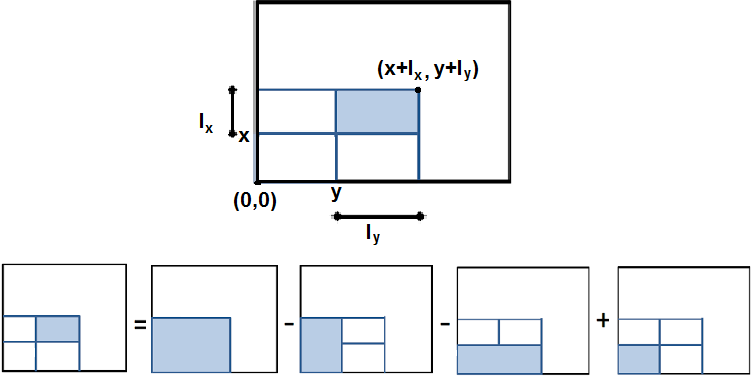
\includegraphics[width=3.5in]{IntegralImages}
	% where an .eps filename suffix will be assumed under latex, 
	% and a .pdf suffix will be assumed for pdflatex; or what has been declared
	% via \DeclareGraphicsExtensions.
	\caption[Integral Image]{Once the Integral Image is constructed, the sum of any rectangular area is calculated in constant time.}
	\label{fig:IntegralImages}
\end{figure}


In this paper, we extend Integral Images to Integral Volumes and use them to quickly identify and ignore big chunks of empty voxels during polygonisation. The following section explains the mathematics behind Integral Volumes, while sections \ref{sec:IVoptApproach}  and \ref{sec:IVcodeDetails} give an in depth description about the algorithms invented. 

\subsubsection{Extending Integral Images to Integral Volumes}\label{sec:extendingIV}

As shown in Figure \ref{fig:IntegralImages},the area of interest is defined by the pixels $(x, y)$ and $(x+l_x, y+l_y)$ and the sum $S$ is given by: 
\begin{equation}
\begin{split}
S = & T(x+l_x,y+l_y) - 
T(x+l_x,y-1)- \\
&  T(x-1,y+l_y) +
T(x-1,y-1)
\end{split}
\label{eq:IntegralImage}
\end{equation}

where 	$S$ is the sum of rectangular area of interest, $T(x, y)$ is the value of the integral image at $(x, y)$ and $l_x, l_y$ define the length of the rectangle in the x and y axis respectively. 

Extending integral images to 3D, the value of the voxel $(x ,y, z)$ in a 3D integral volume becomes equal to the sum of all the values that belong to the box defined by the $(x, y, z)$ and $(0, 0, 0)$ included. 
Therefore the sum $(S)$ of the box defined by $(x, y, z)$ and $(x+l_x, y+l_y, z+l_z)$ included is given by:
\begin{equation}
\begin{split}
S = & T(x-l_x,y+l_y,z+l_z) - 
T(x-1,y+l_y,z+l_z) - \\
&  T(x+l_x,y-1,z+l_z) - 	
T(x+l_x,y+l_y,z-1) + \\
&  T(x-1,y-1,z+l_z)   +
T(x-1,y+l_y,z-1)   +  \\
&  T(x+l_x,y-1,z-1)   -
T(x-1,y-1,z-1)
\end{split}
\end{equation}

where 	$T(x, y, z)$ is the value of the voxel $(x, y, z)$ in the 3D integral volume.  
$S$ is the sum of voxels inside the box, $T(x, y, z)$ is the value of the voxel $(x, y, z)$ in the 3D integral volume. and $l_x, l_y, l_z$ define the length of the box in the $x$, $y$ and $z$ axis respectively. 



\subsubsection{Optimisation Algorithm}\label{sec:IVoptApproach}
As mentioned before, using Integral volumes empty areas are quickly identified and ignored during polygonisation. An iterative algorithm is introduced here. This algorithm continuously splits the volume and checks whether the sub-volumes and its neighbouring voxels are empty using the Integral Volumes. Please note that all the values below the threshold boundary of the object must be zero and all the non-empty voxels must contain a positive value.  

\begin{algorithm}
	\caption{Integral Volumes Optimisation Algorithm}
	\label{alg:IVoptSimple}
	\centering
	\begin{algorithmic}[1]
		\STATE Push the entire Volume as a cuboid inside a Stack
		\WHILE {stack is not empty }
		\STATE Cuboid-A   $\gets$  next cuboid from the Stack 
		\IF{Cuboid-A and neighbours are empty} 
		\STATE	discard Cuboid-A
		\ELSIF { Cuboid-A consists of only one cube}
		\STATE polygonise Cuboid-A
		\ELSE 
		\STATE divide Cuboid-A
		\STATE push the two new Cuboids into stack
		\ENDIF
		\ENDWHILE
	\end{algorithmic}
\end{algorithm}
Here it is worth highlighting that, on line 3 of the algorithm it is checked if the neighbouring cubes of a cuboid are empty (figure 5) as well, because the voxels of the 3D density volume and the cubes in marching cubes algorithm are  aligned with an offset \cite{Miltiadou2015}. If volumes with non-empty neighbouring voxels are ignored, then holes appear on the output polygon mesh. 		

\begin{figure}[!htbp]
	\centering
	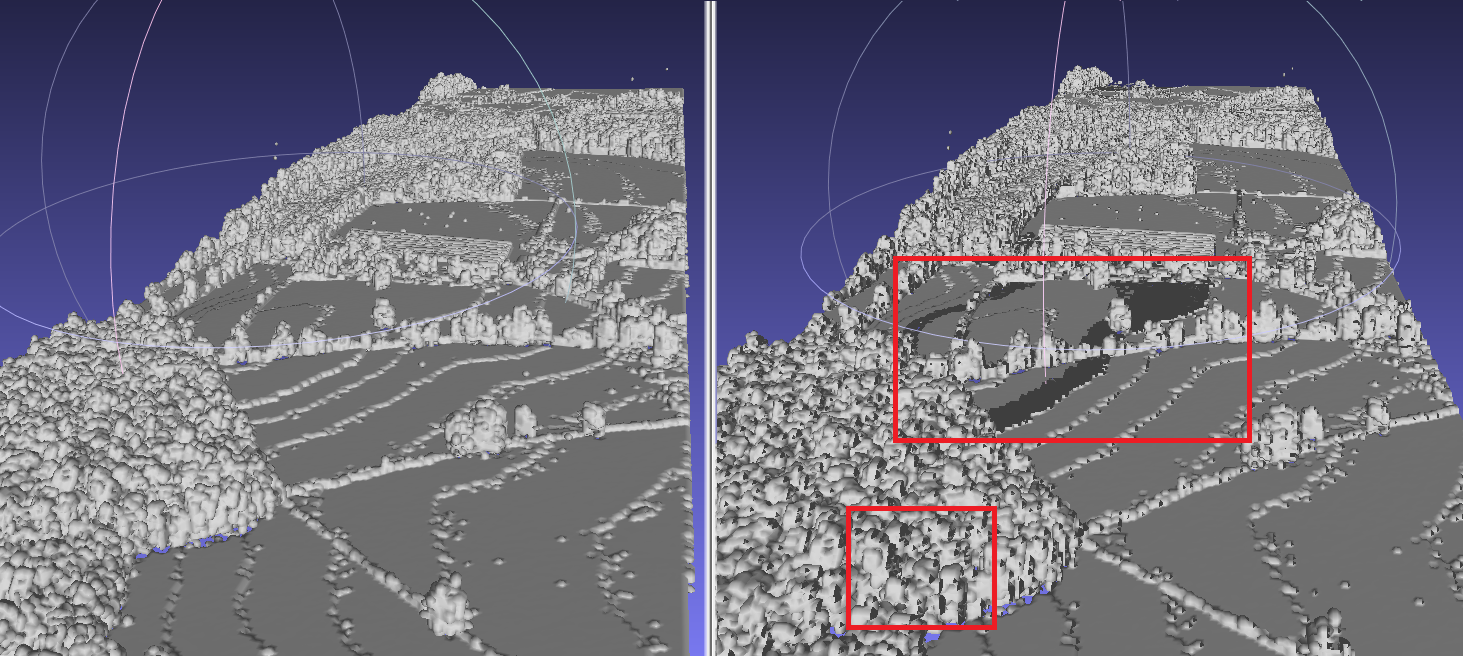
\includegraphics[width=3.5in]{HolesNeighbours}
	% where an .eps filename suffix will be assumed under latex, 
	% and a .pdf suffix will be assumed for pdflatex; or what has been eclared
	% via \DeclareGraphicsExtensions.
	\caption{Comparison between including and ignoring neighborouing voxels; holes appears when ignored.}
	\label{fig:IVholesNeighbours}
\end{figure}

\subsubsection{Coding Details for Faster Implementation}\label{sec:IVcodeDetails}
Implementation details contributes to the efficiency and speed up of the algorithm. Significant improvements are achieved by reducing recursions, big memory allocations and if statements, since memory jumps are time expensive. As shown in algorithm \ref{alg:IVoptSimple}, a while loop is used to avoid recursion. In this section it's given an explanation on how the stack controls memory consumption and how bitwise operations reduces if-statement usage. 

Regarding memory consumption, a stack was chosen over a queue, to decrease the amount of cubes saved into the data structure simultaneously. A queue is a first in first out data structure, while a stack accesses data in a last in first out order. In every iteration, it is ideal to interpret the smallest saved cube, such that the possibility of being polygonised is higher and the possibility of storing another cube is less. A queue guarantees cubes with approximately the same size, since the big cubes will be added first and sequentially being divided first. In contrast, a stack guarantees the smallest possible number of cubes saved. The larger cubes are stored in the bottom of the stack while the smaller ones are interpreted first because they are always the last one divided and inserted into the stack.  For that reason, a stack guarantees the lowest memory usage. 

Furthermore, in algorithm \ref{alg:IVoptSimple} an issue exists: how to quickly identify the side to be divided next? Ideally, the usage of if-statements should be low because they contains many time expensive memory jumps. For that reason, bitwise operations were embedded into the program to reduce their usage. A cube is defined with its position, its size, the next side to be divided $s$ and its divisible sides $D$. The parameter $s$ takes the values $1$, $2$, $3$ for the $x$, $y$, $z$ sides respectively. The parameter $D$ is an integer consisting of the sum of three numbers $(1$ or $0)+(2$ or $0)+(4$ or $0)$ indicating whether the sides  $x$, $y$, $z$ are divisible or not (table \ref{tab:divisiblesNum}). The parameter $D$ takes the value between $[0,7]$ and covering all the possible cases of divisible sides as shown in tables \ref{tab:Dnumbers} and \ref{tab:Dbinary}. For example if $x$ and $z$ are the divisible sides, then $D = 1+0+4 = 5$. By the end, the bitwise operations and the faster implementations of the Integral Volumes optimisations is shown at algorithm \ref{alg:IVoptAdvance}.



\begin{table}[!htbp]
	% increase table row spacing, adjust to taste
	\renewcommand{\arraystretch}{1.3}
	% if using array.sty, it might be a good idea to tweak the value of
	% \extrarowheight as needed to properly center the text within the cells
	\caption{Values of divisible sides}
	\label{tab:divisiblesNum}
	\centering
	% Some packages, such as MDW tools, offer better commands for making tables
	% than the plain LaTeX2e tabular which is used here.
	\begin{tabular}{|P{0.8cm}||P{1.0cm}|P{1.0cm}||P{1.0cm}|P{1.0cm}|}	
		\hline
		&	\multicolumn{2}{c||}{Decimal Numbers} & \multicolumn{2}{c|}{Binary Numbers}  \\
		\hline\hline
		Side &	Divisible & Not Divisible &	Divisible &	Not Divisible  \\
		\hline
		X &	1 &	0 &	0001 &	0000  \\	
		\hline
		Y &	2 &	0 &	0010 &	0000  \\
		\hline
		Z &	4 &	0 &	0100 &	0000 \\
		\hline
	\end{tabular}
\end{table}



\begin{table}[!htbp]
	% increase table row spacing, adjust to taste
	\renewcommand{\arraystretch}{1.3}
	% if using array.sty, it might be a good idea to tweak the value of
	% \extrarowheight as needed to properly center the text within the cells
	\caption{How to calculate the value of D, which represents the divisible sides of a cuboid}
	\label{tab:Dnumbers}
	\centering
	% Some packages, such as MDW tools, offer better commands for making tables
	% than the plain LaTeX2e tabular which is used here.
	\begin{tabular}{|P{0.3cm}||P{0.5cm}|P{0.5cm}|P{0.5cm}|P{0.5cm}|P{0.5cm}|P{0.5cm}|P{0.5cm}|P{0.5cm}|}	
		\hline
		X &	1 &	- &	1 &	- &	1 &	- &	1 &	- \\	
		\hline
		Y &	2 &	2 &	- &	- &	2 &	2 &	- &	- \\
		\hline
		Z &	4 &	4 &	4 &	4 &	- &	- &	- &	- \\
		\hline
		D &	7 &	6 &	5 &	4 &	3 &	2 &	1 &	0 \\
		\hline
	\end{tabular}
\end{table}


\begin{table}[!htbp]
	% increase table row spacing, adjust to taste
	\renewcommand{\arraystretch}{1.3}
	% if using array.sty, it might be a good idea to tweak the value of
	% \extrarowheight as needed to properly center the text within the cells
	\caption{How to calculate the value of divisible sides (D) in binary representation}
	\label{tab:Dbinary}
	\centering
	% Some packages, such as MDW tools, offer better commands for making tables
	% than the plain LaTeX2e tabular which is used here.
	\begin{tabular}{|P{0.3cm}||P{0.5cm}|P{0.5cm}|P{0.5cm}|P{0.5cm}|P{0.5cm}|P{0.5cm}|P{0.5cm}|P{0.5cm}|}
		\hline
		X &	0001 &	-	 &	0001 &	-	 &	0001 &	-	 &	0001 &	-   \\
		\hline
		Y &	0010 &	0010 &	-	 &	-	 &	0010 &	0010 &	-	 &	-   \\
		\hline
		Z &	0100 &	0100 &	0100 &	0100 &	-	 &	-	 &	-	 &	-   \\
		\hline
		D &	0111 &	0110 &	0101 &	0100 &	0011 &	0010 &	0001 &	0000\\
		\hline
	\end{tabular}
\end{table}



\begin{algorithm}[!htbp]
	\caption{Integral Volumes Optimisation Algorithm}
	\label{alg:IVoptAdvance}
	\centering
	\begin{algorithmic}[1]
		\STATE Push the entire Volume as a cuboid inside a Stack
		\WHILE {stack is not empty }
		\STATE Cuboid-A   $\gets$  next cuboid from the Stack 
		\IF{Cuboid-A and neighbours are empty} 
		\STATE	discard Cuboid-A
		\ELSIF { $D$ is equal to $0$}
		\STATE polygonise Cuboid-A
		\ELSIF { $( D$ bitwise add $2^s )$ shift right $(s-1)$ }
		\STATE	divide side s of Cuboid-A 
		
		\IF { the new length of side $s$ is equal to $1$ } 
		\STATE	$D \gets D$ bitwise add $(7-2^s)$
		\ENDIF
		\STATE 	$s \gets (s+1) \text{ mod } 3$
		\STATE push both new Cuboids into stack
		\ELSE 
		\STATE $s \gets (s+1) \text{ mod } 3$
		\STATE push Cuboid-A back into the stack
		
		\ENDIF
		\ENDWHILE
	\end{algorithmic}
\end{algorithm}


\subsection{Octree Max and Min} \label{sec:OctreeMaxMin}



\subsection{Integral Tree}\label{sec:ITopt}
-> 1D Array and Integral Volumes save data coferent memory, making accessing data efficient time but memory alocaton is much higher and because they require continous data to be allocated and all the empty voxels are also included. 

\subsubsection{Constructing the Structure}

\begin{figure}[!htbp]
	\centering
	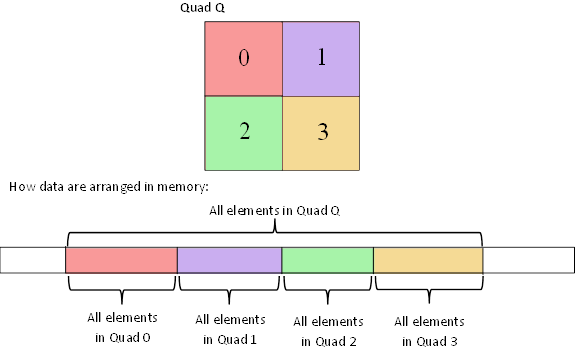
\includegraphics[width=3.5in]{IntegralTree}
	% where an .eps filename suffix will be assumed under latex, 
	% and a .pdf suffix will be assumed for pdflatex; or what has been eclared
	% via \DeclareGraphicsExtensions.
	\caption{Comparison between including and ignoring neighborouing voxels; holes appears when ignored.}
	\label{fig:IntegralTreeQuads}
\end{figure}

\subsubsection{Optimisation Algorithm}






\section{Evaluation and Experiments}


The following tests first test how well each data structure performs in terms of execution time and memory usage. 
Different algorithms could either be beneficial in speeding up the process or decrease memory usage. 

\subsection{Execution Time}
Time program required to be executed
Table single flightline different resolutions



Same resolution, constant noise level, different Flightlines



LDR-FW-FW10\_01-201009821.LA

\section{Results and Discussion}

\section{Results and Discussion}

\begin{table*}[!htbp]
	% increase table row spacing, adjust to taste
	\renewcommand{\arraystretch}{1.3}
	% if using array.sty, it might be a good idea to tweak the value of
	% \extrarowheight as needed to properly center the text within the cells
	\caption{File: LDR-FW-FW10\_01-201009821.LAS Execution Time Results of all the data structures tested. Con for Construction time and Pol for Polygonisation time}
	\label{tab:divisiblesNum}
	\centering
	% Some packages, such as MDW tools, offer better commands for making tables
	% than the plain LaTeX2e tabular which is used here.
	\begin{tabular}{|P{0.7cm}|P{1.6cm}||P{0.65cm}|P{0.65cm}|P{0.65cm}|P{0.65cm}||P{0.65cm}|P{0.65cm}|P{0.65cm}|P{0.65cm}||P{0.65cm}|P{0.65cm}|P{0.65cm}|P{0.65cm}|}	
		\hline\hline
		\multicolumn{2}{|c||}{} & \multicolumn{4}{c||}{1D-array} & \multicolumn{4}{c||}{Voxels Hashing} &\multicolumn{4}{c|}{Octree}  \\
		\hline
		
		\multicolumn{2}{|c||}{Resolution} & \multicolumn{3}{c|}{Time (s)} & \multicolumn{1}{c||} {Memory} & \multicolumn{3}{c|}{Time (s)}&  \multicolumn{1}{c||}{Memory}&\multicolumn{3}{c|}{Time (s)}& \multicolumn{1}{c|}{Memory}  \\
		\hline
		Voxel Length (m) & Number of Voxels & Con & Pol & Total& Max (MB) &  Con & Pol & Total & Max (MB) &  Con & Pol &Total & Max (MB) \\
		\hline\hline
		20 &29x115x23   & 12.04 &0.16 &12.21	& 10.17& 12.84 & 0.19 &13.02 & 9.78 &14.58& 0.18 &14.76& 11.07\\	
		\hline
		15 &39x157x30   & 12.06 &0.32&12.38	& 12.50 & 12.96 &0.37 &13.33 &11.44&14.91 & 0.35 & 15.26 & 12.00\\
		\hline
		10& 58x235x45   & 12.07 & 0.80 &12.87 & 20.09 & 12.95 & 0.96 &13.92 &16.19& 14.92& 0.91 &  15.82& 16.69\\
		\hline
		5&116x476x89    & 12.08 &4.85 &16.92 &88.35	 & 13.01 & 6.95 &19.96 & 47.66& 15.26 & 5.55 & 20.81 &50.50\\
		\hline
		4& 145x597x111  & 12.24 &9.21&21.45  &158.94 & 13.08 &12.83&25.91 &76.7& 15.58& 10.61 & 26.19&  80.31\\
		\hline
		3  & 194x800x148&	 12.19 & 21.90 &34.09 &	362.23 & 13.23 &29.94 &43.16 & 153.27 & 15.67& 24.14 & 39.81& 8.27\\
		\hline
		2  &290x1199x222&	12.45 &67.65 & 80.10	 & 1153.13&	13.69 &95.85 & 109.54 &389.34& 16.16 &75.29& 91.45 & 417.98\\
		\hline
		1.5&387x1602x295& 12.83 & 151.48 & 164.31 &	2666.67 &  13.96 &216.35&230.31 &788.00&16.26 & 166.23&182.49 &839.35 \\
		\hline
		1  &80x2405x443 &	14.62 & 443.5 & 458.1	& 8556.78 &	 15.43 & 672.07 & 687.50 &1912.57 & 16.91& 491.88& 508.79& 2056.805\\
		\hline
		\multicolumn{11}{c}{ } \\
		\hline\hline
		\multicolumn{2}{|c||}{} & \multicolumn{4}{c||}{Integral Volumes} & \multicolumn{4}{c||}{Integral Tree} &\multicolumn{4}{c|}{Octree Max/Min}  \\
		\hline
		
		\multicolumn{2}{|c||}{Resolution} & \multicolumn{3}{c|}{Time (s)} & \multicolumn{1}{c||}{Memory} & \multicolumn{3}{c|}{Time (s)}&  \multicolumn{1}{c||}{Memory}&\multicolumn{3}{c|}{Time (s)}& \multicolumn{1}{c|}{Memory}  \\
		\hline
		Voxel Length (m) & Cubes & Con & Pol & Total& Max (MB) &  Con & Pol & Total & Max (MB) &  Con & Pol &Total & Max (MB) \\
		\hline\hline
		20 &29x115x23    & 12.90 &  0.15 & 13.05 &   10.38 && & & & & & & \\	
		\hline
		15 &39x157x30    & 12.11 &  0.28 & 12.39 &   12.80 && &	& & & & & \\
		\hline
		10 & 58x235x45   & 12.17 &  0.68 & 12.85 &   20.43 && &	& & & & &  \\
		\hline 
		5  &116x476x89   & 13.62 &  3.56 & 16.02 &   88.84 &&&	& & & & &  \\
		\hline
		4  & 145x597x111 & 13.32 & 6.48  & 19.81 &  159.08 && &	& & & & &  \\
		\hline
		3  & 194x800x148 & 15.15 & 14.37 & 29.52 &  363.95 && &	& & & & &  \\
		\hline
		2  &290x1199x222 & 23.11 & 40.80 & 63.91 & 1154.02 && &	& & & & &  \\
		\hline
		1.5&387x1602x295 & 39.64 & 86.54 & 126.18& 2667.67&&&	& & & & &  \\
		\hline
		1  &80x2405x443  & 111.38 &210.94& 322.32& 8559.66&&&	& & & & &  \\
		\hline
		\hline
	\end{tabular}
\end{table*}


\begin{table*}[!htbp]
	% increase table row spacing, adjust to taste
	\renewcommand{\arraystretch}{1.3}
	% if using array.sty, it might be a good idea to tweak the value of
	% \extrarowheight as needed to properly center the text within the cells
	\caption{File: LDR-FW-FW10\_01-201009821.LAS Execution Time Results of all the data structures tested. Con for Construction time and Pol for Polygonisation time}
	\label{tab:divisiblesNum}
	\centering
	% Some packages, such as MDW tools, offer better commands for making tables
	% than the plain LaTeX2e tabular which is used here.
	\begin{tabular}{|P{0.7cm}|P{1.6cm}||P{0.65cm}|P{0.65cm}|P{0.65cm}|P{0.65cm}||P{0.65cm}|P{0.65cm}|P{0.65cm}|P{0.65cm}||P{0.65cm}|P{0.65cm}|P{0.65cm}|P{0.65cm}|}	
		\hline\hline
		\multicolumn{2}{|c||}{} & \multicolumn{4}{c||}{1D-array} & \multicolumn{4}{c||}{Voxels Hashing} &\multicolumn{4}{c|}{Octree}  \\
		\hline
		
		\multicolumn{2}{|c||}{Resolution} & \multicolumn{3}{c|}{Time (s)} & \multicolumn{1}{c||} {Memory} & \multicolumn{3}{c|}{Time (s)}&  \multicolumn{1}{c||}{Memory}&\multicolumn{3}{c|}{Time (s)}& \multicolumn{1}{c|}{Memory}  \\
		\hline
		Voxel Length (m) & Number of Voxels & Con & Pol & Total& Max (MB) &  Con & Pol & Total & Max (MB) &  Con & Pol &Total & Max (MB) \\
		\hline\hline
		6   &    96x250x76 & 5.294 & 0.002 & 5.295 &   40.012 &  5.547 &  0.002 &  5.549 &  21.129 &  6.536 & 0.002 &  6.538 &   22.547  \\	
		3   &  191x561x149 & 5.377 & 0.012 & 5.390 &  237.391 &  5.674 &  0.017 &  5.690 &  80.449 &  6.707 & 0.013 &  6.720 &   83.945  \\	
		1.5 & 381x1122x296 & 5.817 & 0.086 & 5.903 & 1713.738 &  6.120 &  0.127 &  6.247 & 369.613 &  6.856 & 0.091 &  6.949 &  120.565  \\	
		\hline
		6   &   100x760x64 & 22.212 & 0.004 & 22.217 & 84.551 & 23.649 &  0.006 & 23.656 &  48.102 & 31.039 & 0.005 & 31.044 &   52.227  \\	
		3   & 199x1525x124 &22.480 & 0.039 & 22.519 & 608.285 & 24.053 &  0.051 & 24.105 & 281.258 & 30.904 & 0.043 & 30.946 &  292.184  \\		
		1.5 & 398x3063x248 &23.558 & 0.265 &23.823 & 4477.020& 26.190 &  0.372 & 26.563 &1418.922 & 32.137 & 0.293 & 32.431 & 1505.449  \\	
		\hline
		6   &   382x90x108 & 22.433 & 0.003 & 22.435 &62.496 & 24.454 & 0.004 & 24.458 &   29.672 & 32.577 & 0.003 & 32.581 & 32.164\\	
		3   &  763x178x213 &21.953 & 0.018 &21.971  & 397.727 & 23.805 & 0.028 & 23.833 &  126.063 & 32.046 & 0.021 & 32.067 &   37.365\\	
		1.5 & 1526x355x424 & 22.840 & 0.165 & 23.004& 3044.094 & 25.025 & 0.262 & 25.287 &  707.754 & 33.000 & 0.170 & 33.170 &  769.434 \\	
		\hline
		\multicolumn{11}{c}{ } \\
		\hline\hline
		\multicolumn{2}{|c||}{} & \multicolumn{4}{c||}{Integral Volumes} & \multicolumn{4}{c||}{Integral Tree} &\multicolumn{4}{c|}{Octree Max/Min}  \\
		\hline
		
		\multicolumn{2}{|c||}{Resolution} & \multicolumn{3}{c|}{Time (s)} & \multicolumn{1}{c||}{Memory} & \multicolumn{3}{c|}{Time (s)}&  \multicolumn{1}{c||}{Memory}&\multicolumn{3}{c|}{Time (s)}& \multicolumn{1}{c|}{Memory}  \\
		\hline
		Voxel Length (m) & Cubes & Con & Pol & Total& Max (MB) &  Con & Pol & Total & Max (MB) &  Con & Pol &Total & Max (MB) \\
		\hline\hline
		6   &    96x250x76 &  5.501 &  0.001 &  5.503 &    40.05 & & & & & & & & \\	
		3   &  191x561x149 &  7.133 &  0.007 &  7.140 &   237.75 & & & & & & & & \\	
		1.5 & 381x1122x296 & 23.977 &  0.040 & 24.017 &  1714.71 & & & & & & & & \\	
		\hline
		6   &   100x760x64 & 22.691 & 0.003 &  22.695 &   89.902 & & & & & & & & \\	
		3   & 199x1525x124 & 28.044 & 0.026 &  28.070 &  608.785 & & & & & & & & \\		
		1.5 & 398x3063x248 & 69.418 & 0.160 &  69.577 & 4478.664 & & & & & & & & \\	
		\hline
		6   &   382x90x108 & 23.119 & 0.002 &  23.121 &   63.020 & & & & & & & & \\	
		3   &  763x178x213 & 24.525 & 0.010 &  24.535 &  398.164 & & & & & & & & \\	
		1.5 & 1526x355x424 & 62.250 & 0.077 &  62.327 & 3045.414 & & & & & & & & \\	
		\hline
		\hline
	\end{tabular}
\end{table*}


\section{Conclusion}
The Hashed Octree approach could further be used for speeding up neighbouring search in spatial representation of geometric objects.

\end{document}